\section{Snake robot kinematics}\label{sec:kin}


The snake robot is modeled as a serial chain, which is a system of rigid bodies in which each member is connected to two others, except for the first and last members that are each connected to only one other member \cite{waldron2016kinematics}. As opposed to traditional robot manipulator models, the first joint in the snake robot model is not physically connected to a base.


The vector of generalized coordinates $\mathbf{q}$ for a snake robot with $n$ links is

\begin{equation} \label{eq:q}
    \mathbf{q} = 
    \begin{bmatrix}
        \phi_1 & \phi_2 & ... & \phi_n & x_0 & y_0
    \end{bmatrix}^T.
\end{equation}
\\
The coordinates $(x_0, y_0)$ and $\phi_1$ represent the position and orientation of the tail of the snake robot in reference to the base frame $(x,y)$. These coordinates cannot be directly controlled and will therefore be referred to as virtual coordinates. The generalized coordinates ${\phi_2, ... ,  \phi_n}$, corresponding to the actuated joints, refer to the angle of the following link relative to the preceding link. The number of generalized coordinates including two position coordinates and $n$ joint angles is $N = n+2$.

The model of the snake robot with the named variables are illustrated in Figure \ref{fig:kin_name}. 
\begin{figure}
    \centering
    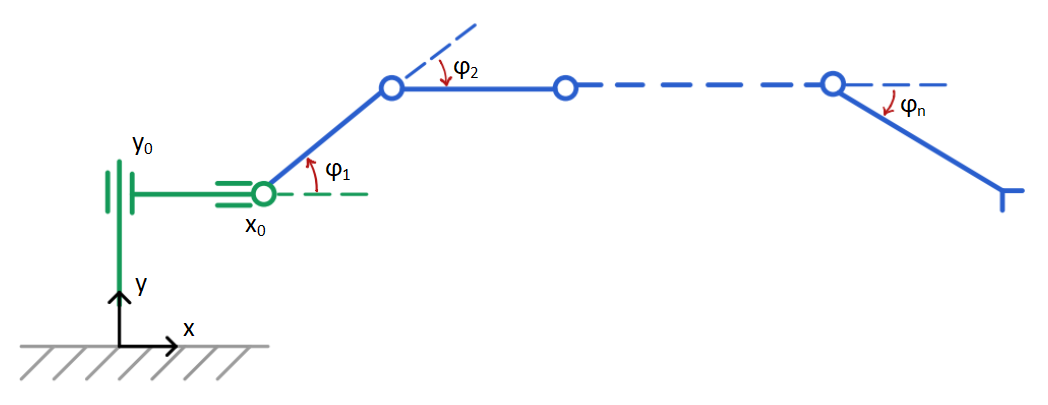
\includegraphics[width=0.9\textwidth]{figures/theory/kinematics.PNG}
    \caption{Model of snake robot with notation}
    \label{fig:kin_name}
\end{figure}


Homogeneous transformation matrices are used to express the pose (position and orientation) of the links in relation to the base frame. This means that as long as the joint angles and size of the snake robot are known, the Cartesian positions can be calculated.
The homogeneous transformation matrix for the end point of link $i$ from the base frame $b$ is given by (\ref{eq:transformationmatrix}). The base frame will stay put regardless of motion of the robot. Note also that the link length $l$ is assumed equal for all the links.

\begin{equation} \label{eq:transformationmatrix}
    \textbf{T}_{b i} = \textbf{D}_x(x_0) \textbf{D}_y(y_0) \sum_{k=1}^{i} \textbf{R}_z(\phi_k) \textbf{D}_x(l)
\end{equation}
\\
The translation and rotation matrices are given by

\begin{equation}\label{eq:trans_rot}
    \begin{split}
        \textbf{D}_x(x)& = 
        \begin{bmatrix}
            1 & 0 & x \\
            0 & 1 & 0 \\
            0 & 0 & 1
        \end{bmatrix}, \ \
        \textbf{D}_y(y) =
        \begin{bmatrix}
            1 & 0 & 0 \\
            0 & 1 & y \\
            0 & 0 & 1
        \end{bmatrix}, \ \
        \\&
        \\&\textbf{R}_z(\phi) =
        \begin{bmatrix}
            \cos{\phi} & -\sin{\phi} & 0 \\
            \sin{\phi} &  \cos{\phi} & 0 \\
            0          &  0          & 1
        \end{bmatrix}.
    \end{split}
\end{equation}
\\
The transformation matrix from the reference frame to the center of link $i$ can be found in the same manner. The only difference is that the very last translational matrix has to take the argument $l/2$ instead of $l$. This is useful to keep in mind as it be used in Section \ref{sec:dyn} for the derivation of the kinetic energy of the links.

As mentioned earlier, the transformation matrix $\textbf{T}_{b i}$ can be used to find the absolute orientation and position of the tip of link $i$ in the base frame.
The resulting matrix can be written on the form

\begin{equation}
    \textbf{T}_{b i} =
    \NORMAL{
    \begin{bmatrix}
        \textbf{R}_{b i}(\phi_{i,abs}) & \textbf{t}_{r i}^r \\
        \textbf{0}^T & 1
    \end{bmatrix} }.
\end{equation}
\\
The position is directly extracted from $\textbf{t}_{r i}^r = [x_i y_i]^T$. The orientation $\phi_{i,abs}$ is found by comparing $\textbf{R}_{b i}$ to $\textbf{R}_z$ and solving for $\phi_{i,abs}$.

Alternatively, one can directly compute the position of the center of a link $i$ from the expressions below

\begin{equation} \label{eq:pos}
    \begin{split}
        x_i &= x_0 + \sum_{k=1}^{i} l \cos{(\sum_{j=1}^{k} \phi_j)} \\
        y_i &= y_0 + \sum_{k=1}^{i} l \sin{(\sum_{j=1}^{k} \phi_j)},
    \end{split}
\end{equation}
\\
where $l$ is the link length and $1\leq i\leq n$.

\subsubsection{Forward and inverse instantaneous kinematics}\label{subseq:inst_fwd}

The well known Jacobian lets us transform between Cartesian and joint velocities. It is derived by taking the partial derivative of the $x$ and $y$ position of link $1\leq i\leq n$ with respect to all generalized coordinates

\begin{equation}\label{eq:Jc1}
    \mathbf{J_i} = 
    \HUGE{
    \begin{bmatrix}
        \frac{\partial x_i}{\partial q_1} & ... & \frac{\partial x_i}{\partial q_{N-1}} & \frac{\partial x_i}{\partial q_{N}} \\
        \frac{\partial y_i}{\partial q_1} & ... & \frac{\partial y_i}{\partial q_{N-1}} & \frac{\partial y_i}{\partial q_{N}} \\
    \end{bmatrix}
    }.
\end{equation}
\\
The relationship between the Cartesian velocity $\mathbf{v}$ of the point $(x_i, y_i)$ on the robot and the joint velocities $\mathbf{\dot{q}}$ can thus be written as 

\begin{equation}
    \mathbf{v_i = J_i(q) \dot{q}} \quad \textrm{ and } \quad \mathbf{\dot{q} = J_i(q)^\dagger v_i}.
\end{equation}
\\
The first equation is formally referred to as the forward instantaneous kinematics, whereas the second one is referred to as the inverse instantaneous kinematics.
$\mathbf{J(q)^\dagger}$ is the pseudo inverse of the Jacobian, which has to be used as a result of the Jacobian being non-square.

%------------------------------------------------------------------------------------------------

\subsection{Constrained kinematics}\label{seq:constr_kin}

%\hl{Virtual closed kinematic chain}\\
For the case in which the robot is in contact with the environment, the motion will be constrained. The obstacles found in the environment are modelled as single frictionless points. The only constraint imposed by the environment is that the robot cannot penetrate the obstacles. It can, however, both apply an arbitrary large force against them or move along them.

The model assumes that any link can be in contact with at most one obstacle at the time. To represent the mentioned constraint, the vector of generalized coordinates is expanded with $n$ further elements, where $n$ is the number of links. The updated vector $\mathbf{q}$ is now

\begin{equation} \label{eq:q2}
    \mathbf{q} = 
    \begin{bmatrix}
        \phi_1 & \phi_2 & ... & \phi_n & x_0 & y_0 & d_{c,1} & d_{c,2} & ... & d_{c,n}
    \end{bmatrix}^T,
\end{equation}
\\
where $N = 2 + 2n$ is the new number of generalized coordinates.

The newly introduced coordinates $d_{c,1}, ... , d_{c,n} \geq 0$ represent the distance to the possible contact point from the corresponding joint. For instance, the coordinate $d_{c,2}$ is the distance between the second joint and the contact point measured along the second link, as illustrated in Figure \ref{fig:3_obs_force}. Every link might not be in contact with an obstacle, but the maximum number of coordinates is introduced in the interest of keeping the vector size constant. 
Seeing as there is no actuation force directly connected to the obstacle-related coordinates, they will be referred to as virtual joints or virtual coordinates.

The position of a contact point on link $1\leq i\leq n$ in the base frame can be derived through the corresponding transformation matrix (\ref{eq:obst_tfmatrix}).

\begin{equation} \label{eq:obst_tfmatrix}
    \textbf{T}_{b ci} = \textbf{D}_x(x_0) \textbf{D}_y(y_0) \sum_{k=1}^{i-1} (\textbf{R}_z(\phi_k) \textbf{D}_x(l)) \textbf{R}_z(\phi_i) \textbf{D}_x(d_{c,1})
\end{equation}

\begin{figure}
    \centering
    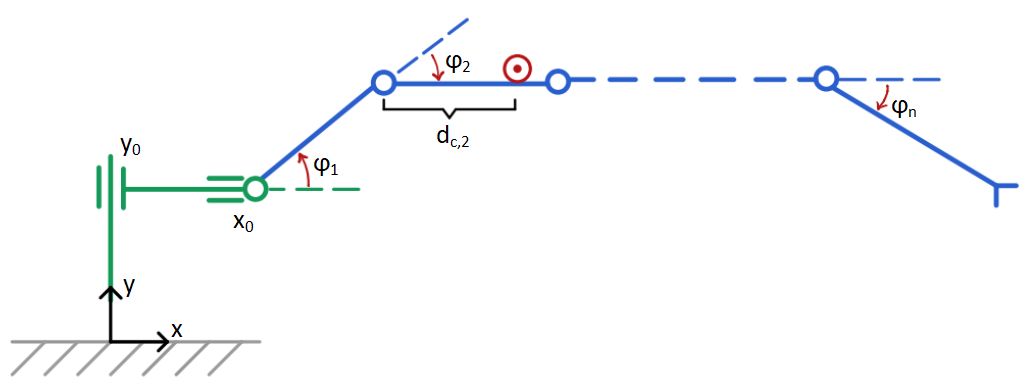
\includegraphics[width=0.9\textwidth]{figures/theory/contact_point.PNG}
    \caption{Snake robot in contact with obstacle}
    \label{fig:3_obs_force}
\end{figure}


%------------------------------------------------------------------------------------------------

\subsubsection{Constrained instantaneous kinematics}\label{subseq:constr_inst}

The Jacobian matrix related to the velocity of the contact point can be derived in the same manner as in the unconstrained case. The only difference is that the partial differentiation of the contact point $(x_c,y_c)$ is now taken with respect to the extended vector of generalized coordinates (\ref{eq:q2}). The resulting contact Jacobian for a contact point on link $1\leq i\leq n$ is thus

\begin{equation}\label{eq:Jac_constr}
    J_{c,i} = 
    \HUGE{
    \begin{bmatrix}
        \frac{\partial x_{c,i}}{\partial \phi_2} & ... & \frac{\partial x_{c,i}}{\partial q_{N-1}} & \frac{\partial x_{c,i}}{\partial q_N} \\
        \frac{\partial y_{c,i}}{\partial \phi_2} & ... & \frac{\partial y_{c,i}}{\partial q_{N-1}} & \frac{\partial y_{c,i}}{\partial q_N} \\
    \end{bmatrix}
    }.
\end{equation}
\\
This Jacobian will end up being quite sparse, seeing as the coordinate of a contact point is independent of all other contact coordinates. This is a property that can be exploited using sparse solvers if the snake robot has a large number of links.

The relationships between the Cartesian velocity of a contact point on link $1\leq i\leq n$ and the joint velocities can now be expressed as

\begin{equation}
    \mathbf{v_{c,i} = J_{c,i}(q) \dot{q}} \quad \textrm{ and } \quad \mathbf{\dot{q} = J_{c,i}(q)^\dagger v_{c,i}}.
\end{equation}

